\section{Testing JUnit}

\lstset{
tabsize = 4, %% set tab space width
showstringspaces = false, %% prevent space marking in strings, string is defined as the text that is generally printed directly to the console
numbers = left, %% display line numbers on the left
commentstyle = \color{green}, %% set comment color
keywordstyle = \color{blue}, %% set keyword color
stringstyle = \color{red}, %% set string color
rulecolor = \color{black}, %% set frame color to avoid being affected by text color
basicstyle = \small \ttfamily, %% set listing font and size
breaklines = true, %% enable line breaking
numberstyle = \tiny,
}
 

\begin{flushleft}

    In questa sezione, presentiamo una delle fasi cruciali all'interno del ciclo di sviluppo del software, ovvero il testing. 
    Il testing può assumere diverse forme e tipologie, ma per la semplicità della presentazione, in questa sede si richiede
    il testing di soli 4 metodi con due o più parametri, che verrà effettuato mediante l'utilizzo del framework JUnit 5.
\end{flushleft}


%PRIMO METODO

\subsection{Test funzione check credenziali}
\begin{flushleft}
    
    Il metodo \textit{checkCredentials} ha il compito di verificare la validità di un indirizzo email
     e di una password. In particolare, il metodo accetta due stringhe come input: \textit{mail}, che 
     rappresenta l'indirizzo email, e \textit{pswrd}, che rappresenta la password.
    Il metodo restituisce un oggetto \textit{ArrayList} di interi, che rappresenta una 
    lista di eventuali errori verificatisi durante l'esecuzione del metodo. In altre parole, 
    il metodo controlla se l'indirizzo email e la password rispettano determinati requisiti, 
    e in caso contrario, aggiunge il corrispondente codice di errore alla lista.
    Infine, il metodo restituisce la lista degli errori, eventualmente vuota se non sono stati riscontrati problemi.\\
\end{flushleft}

\vspace{0.2cm}

\begin{lstlisting}[language = Java , frame = trBL , firstnumber = last , escapeinside={(*@}{@*)}, commentstyle=\color{brown}]

    public class CheckCredentialsTest {

    /*
    CLASSI DI EQUIVALENZA:
   
    PASSWORD: {VALIDA, VUOTA, TROPPO CORTA, NON RISPETTA LA REGEX}
      - VALIDA = Almeno 8 caratteri di cui 1 Maiuscola,
      1 Minuscola, 1 Carattere speciale, 1 numero

    EMAIL: {VALIDA, VUOTA, NON VALIDA}
      - VALIDA = Deve rispettare la sintassi
      di un email corretta

--------------------------------------------------------------------------------

    CODICI DI ERRORE:
      9 = PASSWORD VUOTA,
      10 = PASSWORD TROPPO CORTA,
      11 = PASSWORD NON VALIDA (REGEX)
      12 = EMAIL VUOTA, 
      13 = EMAIL NON VALIDA

---------------------------------------------------------------------------------

    STRATEGIE DI TESTING UTILIZZATE: 
      BlackBox secondo il criterio SECT

    CASI DI TESTING INDIVIDUATI: 
      22 in 12 metodi

------------------------------------------------------------------------------ */

    public ArrayList<Integer> codici_errore = new ArrayList<Integer>();

    @AfterEach
    public void clearArrayList() {
        codici_errore.clear();
    }

    @Test
    public void testCheckCredentials(){
        assertEquals(codici_errore, checkCredentials("ser.dimartino@studenti.unina.it", "Password.123"));
    }

    @Test
    public void tesPasswordVuota(){
        codici_errore.add(9);
        assertAll(
                () -> assertEquals(codici_errore, checkCredentials("fra.cutugno@studenti.unina.it", null)),
                () -> assertEquals(codici_errore, checkCredentials("lu.starace@studenti.unina.it", ""))
        );
    }

    @Test
    public void testPasswordTroppoCorta(){
        codici_errore.add(10);
        assertEquals(codici_errore, checkCredentials("gio.cutolo@studenti.unina.it", "Aa_09."));
    }

    @Test
    public void testPasswordNonValida(){
        codici_errore.add(11);
        assertAll(
                () -> assertEquals(codici_errore, checkCredentials("alb.aloisio@studenti.unina.it", "password?123")),  // MANCA LA MAIUSCOLA
                () -> assertEquals(codici_errore, checkCredentials("an.corazza@studenti.unina.it", "PASSWORD#123")),  //MANCA LA MINUSCOLA
                () -> assertEquals(codici_errore, checkCredentials("alb.aloisio@studenti.unina.it", "Password123")),  // MANCA IL CARATTERE SPECIALE
                () -> assertEquals(codici_errore, checkCredentials("an.corazza@studenti.unina.it", "Password_unoduetre")) // MANCA IL NUMERO
        );

    }

    @Test
    public void testEmailVuota(){
        codici_errore.add(12);
        assertAll(
                () -> assertEquals(codici_errore, checkCredentials(null, "Password.123")),
                () -> assertEquals(codici_errore, checkCredentials("", "Password.123"))
        );
    }

    @Test
    public void testEmaildNonValida(){
        codici_errore.add(13);
        assertAll(
                () -> assertEquals(codici_errore, checkCredentials("emailcompletamentesbagliata", "Password.123")),  // EMAIL COMPLETAMENTE SBAGLIATA
                () -> assertEquals(codici_errore, checkCredentials("@gmail.com", "Password.123")),  // MANCA LO USERNAME
                () -> assertEquals(codici_errore, checkCredentials("biagio@.net", "Password.123")),  // MANCA IL SECOND LEVEL DOMAIN
                () -> assertEquals(codici_errore, checkCredentials("matteo@libero.", "Password.123")), // MANCA IL TOP LEVEL DOMAIN
                () -> assertEquals(codici_errore, checkCredentials("luigivirgilio.it", "Password.123")), //MANCA LA @
                () -> assertEquals(codici_errore, checkCredentials("MATTEO[BIAGIO]LUIGI_@libero.IT", "Password.123")) // LO USERNAME PRESENTA CARATTERI NON CORRETTI
        );
    }

    @Test
    public void testErroriMultipli_9_12(){
        codici_errore.add(9);
        codici_errore.add(12);

        assertEquals(codici_errore, checkCredentials("", ""));
    }

    @Test
    public void testErroriMultipli_9_13(){
        codici_errore.add(9);
        codici_errore.add(13);

        assertEquals(codici_errore, checkCredentials("@studenti.@libero@com", ""));
    }

    @Test
    public void testErroriMultipli_10_12(){
        codici_errore.add(10);
        codici_errore.add(12);

        assertEquals(codici_errore, checkCredentials("", "Ab.34"));
    }

    @Test
    public void testErroriMultipli_10_13(){
        codici_errore.add(10);
        codici_errore.add(13);

        assertEquals(codici_errore, checkCredentials("emailcompletamentesbagliata", "Ab.34"));
    }

    @Test
    public void testErroriMultipli_11_12(){
        codici_errore.add(11);
        codici_errore.add(12);

        assertEquals(codici_errore, checkCredentials("", "Password.Password"));
    }

    @Test
    public void testErroriMultipli_11_13(){
        codici_errore.add(11);
        codici_errore.add(13);

        assertEquals(codici_errore, checkCredentials("@studenti.@libero@com", "@studenti.it"));
    }
}

\end{lstlisting}



%SECONDO METODO
\subsection{Test funzione che calcola incasso in un range di date.}
\begin{flushleft}
   La funzione "getIncassoRangeGiorni" prende in input una data di inizio e una lista di ordini e calcola l'incasso totale degli ordini che sono stati effettuati tra la data di inizio e la data attuale.

    La funzione controlla che la lista degli ordini non sia nulla. In caso contrario, restituisce zero. Successivamente, per ogni ordine nella lista degli ordini, la funzione controlla se la data dell'ordine è compresa tra la data di inizio e la data attuale. Se la data è compresa nel range, l'importo dell'ordine viene aggiunto all'incasso totale.
    
    Infine, la funzione restituisce l'incasso totale degli ordini effettuati nel range di tempo specificato.
\end{flushleft}
\vspace{0.2cm}

\begin{flushleft}
    Dato che la funzione "getIncassoRangeGiorni" fa parte della classe StatisticsActivity e fa uso della classe Ordini,
    abbiamo creato nel Package "Driver" i seguenti \textit{Mock} per poter eseguire il testing:
\end{flushleft}
\vspace{1cm}

\begin{lstlisting}[language = Java , frame = trBL , firstnumber = last , escapeinside={(*@}{@*)} , commentstyle=\color{brown}]
    public class StatisticsActivityMock {

    public float media(int giorni, float incasso){
        float media = 0;
        if(giorni < 0) throw new IllegalArgumentException("Il numero di giorni non deve essere negativo");
        if (giorni == 0) throw new ArithmeticException("Il numero di giorni non puo essere 0");
        if (incasso < 0) throw new IllegalArgumentException("l'incasso deve essere maggiore di 0.");
        media = incasso / giorni;
        media = Math.round(media * 100) / 100f;

        return media;
    }

    public int getIncassoRangeGiorni(LocalDate dataInizio, ArrayList<OrdineMock> orders){
        int incassoTotale = 0;
        LocalDate endDate = LocalDate.now();
        DateTimeFormatter formatter = DateTimeFormatter.ofPattern("yyyy-MM-dd");

        if (orders == null) return 0;
        for (OrdineMock ordine : orders) {
            LocalDate orderDate = LocalDate.parse(ordine.getDataOrdine(), formatter);
            if (orderDate.isEqual(dataInizio) || orderDate.isAfter(dataInizio) && orderDate.isBefore(endDate)) {
                incassoTotale += ordine.getConto();


            }
        }
        return incassoTotale;
    }
}
\end{lstlisting}
\vspace{0.2cm}

\begin{lstlisting}[language = Java , frame = trBL , firstnumber = last , escapeinside={(*@}{@*)} , commentstyle=\color{brown}]
   
 /*
    IN QUESTO CASO LA CLASSE ORDINE MOCK CONTIENE SOLO
    GLI ATTRIBUTI DI ORDINE CHE ENTRANO IN GIOCO ALL'INTERNO
    DEL METODO getIncassoRangeGiorni
*/

public class OrdineMock {

   private int conto;
   private String dataOrdine;

   public OrdineMock(int conto, String dataOrdine) {
       this.conto = conto;
       this.dataOrdine = dataOrdine;
   }

   public int getConto() {
       return conto;
   }

   public String getDataOrdine() {
       return dataOrdine;
   }
}

\end{lstlisting}
\vspace{0.2cm}
    
\begin{lstlisting}[language = Java , frame = trBL , firstnumber = last , escapeinside={(*@}{@*)} , commentstyle=\color{brown}]

/*
   CLASSI DI EQUIVALENZA:
   
      DATA_INIZIO: {VALIDA, NULL}
        - Valida: a sua volta puo' essere
             1.1) Verosimile e precedente agli ordini
             1.2) Futura agli ordini
             1.3) Inverosimilmente precedente agli ordini

      ORDINI: {VALIDI, NULL, LISTA VUOTA, CON DATA SBAGLIATA}

 --------------------------------------------------------------------------------

   STRATEGIE DI TESTING UTILIZZATE:

      BlackBox secondo il criterio WECT
      
   CASI DI TESTING RITENUTI NECESSARI:
     {VALIDA , VALIDI} : 1 Caso
     {VALIDA , NULL} : 1 Caso
     {VALIDA , LISTA VUOTA} : 1 Caso
     {VALIDA , CON DATA SBAGLIATA} : 4 Casi
     {DATA FUTURA , VALIDI} : 1 Caso
     {DATA INVEROSIMILMENTE PRECEDENTE , VALIDI} : 1 Caso
     {NULL , VALIDI} : 1 Caso

 ------------------------------------------------------------------------------ */  

public class getIncassoRangeGiorniTest {

    StatisticsActivityMock statisticsActivityMock;
    ArrayList<OrdineMock> ordiniM;
    DateTimeFormatter formatter;

    @Before
    public void setUp(){
        statisticsActivityMock = new StatisticsActivityMock();
        ordiniM = new ArrayList<>();
        formatter = DateTimeFormatter.ofPattern("yyyy-MM-dd");
    }

    @AfterEach
    public void clearArrayList(){
        ordiniM.clear();
    }


    @Test
    public void testGetIncassoRangeGiorni() {
        ordiniM.add(new OrdineMock(3, "2023-05-04"));
        ordiniM.add(new OrdineMock(105, "2023-05-04"));
        ordiniM.add(new OrdineMock(72, "2023-02-04"));

        LocalDate dataInizio = LocalDate.parse("2023-02-05", formatter);

        int result = statisticsActivityMock.getIncassoRangeGiorni(dataInizio, ordiniM);
        assertEquals(108, result);
    }

    @Test
    public void testZeroOrdini()  {
        LocalDate dataInizio = LocalDate.parse("2023-02-01", formatter);

        int result = statisticsActivityMock.getIncassoRangeGiorni(dataInizio, ordiniM);
        assertEquals(0, result);

    }

    @Test
    public void testOrdiniNull()  {
        LocalDate dataInizio = LocalDate.parse("2023-02-01", formatter);

        int result = statisticsActivityMock.getIncassoRangeGiorni(dataInizio, null);
        assertEquals(0, result);

    }

    @Test
    public void testDataInizioNull()  {
        ordiniM.add(new OrdineMock(3, "2023-05-04"));
        ordiniM.add(new OrdineMock(105, "2023-05-04"));
        ordiniM.add(new OrdineMock(72, "2023-02-04"));

        assertThrows(NullPointerException.class,
                () -> statisticsActivityMock.getIncassoRangeGiorni(null, ordiniM));
    }

    @Test
    public void testDataInizioFutura() {
        ordiniM.add(new OrdineMock(3, "2023-05-04"));
        ordiniM.add(new OrdineMock(105, "2023-05-04"));
        ordiniM.add(new OrdineMock(72, "2023-02-04"));

        LocalDate dataInizio = LocalDate.parse("2033-02-05", formatter);

        int result = statisticsActivityMock.getIncassoRangeGiorni(dataInizio, ordiniM);
        assertEquals(0, result);
    }

    @Test
    public void testDataInizioIrrealistica() {
        ordiniM.add(new OrdineMock(3, "2023-05-04"));
        ordiniM.add(new OrdineMock(105, "2023-05-04"));
        ordiniM.add(new OrdineMock(72, "2023-02-04"));

        LocalDate dataInizio = LocalDate.parse("0133-02-05", formatter);

        int result = statisticsActivityMock.getIncassoRangeGiorni(dataInizio, ordiniM);
        assertEquals(180, result);
    }

    @Test
    public void testDataOrdiniInFormatoSbagliato(){
        ArrayList<OrdineMock> ordiniM_1 = new ArrayList<>();
        ArrayList<OrdineMock> ordiniM_2 = new ArrayList<>();
        ArrayList<OrdineMock> ordiniM_3 = new ArrayList<>();
        ArrayList<OrdineMock> ordiniM_4 = new ArrayList<>();

        ordiniM_1.add(new OrdineMock(3, "2023"));
        ordiniM_2.add(new OrdineMock(105, "02/05/2023"));
        ordiniM_3.add(new OrdineMock(72, "due-aprile-2023"));
        ordiniM_4.add(new OrdineMock(105, "2023-32-31"));


        LocalDate dataInizio = LocalDate.parse("2023-02-01", formatter);

        assertAll(
                () ->   assertThrows(DateTimeParseException.class,
                        () -> statisticsActivityMock.getIncassoRangeGiorni(dataInizio, ordiniM_1)
                ),
                () ->   assertThrows(DateTimeParseException.class,
                        () ->statisticsActivityMock.getIncassoRangeGiorni(dataInizio, ordiniM_2)
                ),
                () ->   assertThrows(DateTimeParseException.class,
                        () -> statisticsActivityMock.getIncassoRangeGiorni(dataInizio, ordiniM_3)
                ),
                () ->   assertThrows(DateTimeException.class,
                        () -> statisticsActivityMock.getIncassoRangeGiorni(dataInizio, ordiniM_4)
                )

        );
        ordiniM_1.clear();
        ordiniM_2.clear();
        ordiniM_3.clear();
        ordiniM_4.clear();
    }

}

\end{lstlisting}


%TERZO METODO

\subsection{Test funzione che controlla i campi di un ristorante.}
\begin{flushleft}
    Questo metodo prende in input quattro stringhe che rappresentano il nome di un ristorante,
     il numero di coperti, l'indirizzo' e il numero di telefono. Il metodo restituisce un oggetto ArrayList
     di interi che rappresenta una lista di eventuali errori verificatisi durante l'esecuzione del metodo.
\end{flushleft}
\vspace{0.2cm}

\begin{lstlisting}[language = Java , frame = trBL , firstnumber = last , escapeinside={(*@}{@*)} , commentstyle=\color{brown}]
public class getRestaurantFiedlsErrorsTest {
/*
    CLASSI DI EQUIVALENZA:
 
       NOME: {VALIDO, VUOTO, TROPPO CORTO}
 
       COPERTI: {VALIDO, VUOTO, FUORI-RANGE, NON VALIDO}
         - FUORI RANGE: <5 && > 1000
         - NON VALIDO: Non composto da soli numeri
 
       INDIRIZZO: {VALIDO, VUOTO, TROPPO CORTO, NON VALIDO}
         - NON VALIDO: Contiene caratteri speciali
 
       TELEFONO: {VALIDO, VUOTO, NON VALIDO}
 
  --------------------------------------------------------------------------------
 
    CODICI DI ERRORE:
     1 = NOME TROPPO CORTO (1 CARATTERE MINIMO)
     2 = NOME MANCANTE
     3 = NUMERO DI COPERTI MANCANTE
     4 = NUMERO DI COPERTI FUORI RANGE
     5 = INDIRIZZO MANCANTE
     6 = INDIRIZZO TROPPO CORTA (MINIMO 5 CARATTERI)
     7 = NUMERO DI TELEFONO MANCANTE
     8 = NUMERO DI TELEFONO NON VALIDO (10 CIFRE NUMERICHE RICHIESTE)
     9 = NUMERO DI COPERTI ERRATO
     10 = INDIRIZZO NON VALIDO
 
 -------------------------------------------------------------------------------------
 
    STRATEGIE DI TESTING UTILIZZATE:
       BlackBox secondo il criterio WECT
 
    CASI DI TESTING RITENUTI NECESSARI:
      {VALIDO, VALIDO, VALIDO, VALIDO} : 1 Caso
      {TROPPO CORTO, VALIDO, VALIDO, VALIDO} : 1 Caso
      {VALIDO, FUORI-RANGE, VALIDO, VALIDO} : 2 Casi
      {VALIDO, NON VALIDO, VALIDO, VALIDO} : 2 Casi
      {VALIDO, VALIDO, TROPPO CORTO, VALIDO} : 1 Caso
      {VALIDO, VALIDO, NON VALIDO, VALIDO} : 1 Caso
      {VALIDO, VALIDO, VALIDO, NON VALIDO} : 1 Caso
      {NULL, NULL, NULL, NULL} : 1 Caso
 
  ---------------------------------------------------------------------------- */
    public ArrayList<Integer> codici_errore = new ArrayList<Integer>();


    // L'ARRAYLIST DEVE ESSERE PULITO OGNI VOLTA CHE VIENE CONCLUSO UN CASO DI TEST
    @AfterEach
    public void clearArrayList(){
        codici_errore.clear();
    }

    @Test
    public void testgetRestaurantFieldsError(){
        ArrayList<Integer> actualErrors = getRestaurantFieldsErrors("Ristorante Test", "10", "Via Roma 1", "0123456789");
        assertEquals(codici_errore, actualErrors); //Funziona poiche non ci sono codici di errore: l'ArrayList risulta vuoto
    }

    @Test
    public void testNomeCampoTroppoCorto() {
        codici_errore.add(1);
        ArrayList<Integer> actualErrors = getRestaurantFieldsErrors("a", "10", "Via Roma 1", "0123456789");
        assertEquals(codici_errore, actualErrors);
    }

    @Test
    public void testCampoCopertiFuoriRange(){
        codici_errore.add(4);
        assertAll(
                () -> assertEquals(codici_errore, getRestaurantFieldsErrors("Ristorante Test", "1", "Via Roma 1", "0123456789")),
                () -> assertEquals(codici_errore, getRestaurantFieldsErrors("Ristorante Test", "100000", "Via Roma 1", "0123456789"))
        );
    }

    @Test
    public void testCampoCopertiNonValido(){
        codici_errore.add(9);
        assertAll(
                () -> assertEquals(codici_errore, getRestaurantFieldsErrors("Ristorante Test", "dieci", "Via Roma 1", "0123456789")),
                () -> assertEquals(codici_errore, getRestaurantFieldsErrors("Ristorante Test", "10a", "Via Roma 1", "0123456789"))
        );
    }


    @Test
    public void testLocazioneCampoTroppoCorto() {
        codici_errore.add(6);
        ArrayList<Integer> actualErrors = getRestaurantFieldsErrors("Ristorante Test", "10", "Via", "0123456789");
        assertEquals(codici_errore, actualErrors);
    }

    @Test
    public void testLocazioneNonValido() {
        codici_errore.add(10);
        ArrayList<Integer> actualErrors = getRestaurantFieldsErrors("Ristorante Test", "10", "Via_Napoli?", "0123456789");
        assertEquals(codici_errore, actualErrors);
    }


    @Test
    public void testNumeroTelefonoCampoTroppoCorto() {
        codici_errore.add(8);
        ArrayList<Integer> actualErrors = getRestaurantFieldsErrors("Ristorante Test", "10", "Via Roma 1", "12345678");
        assertEquals(codici_errore, actualErrors);
    }

    @Test
    public void testTuttiICampiVuoti() {
        codici_errore.add(2);
        codici_errore.add(3);
        codici_errore.add(5);
        codici_errore.add(7);
        ArrayList<Integer> actualErrors = getRestaurantFieldsErrors("", "", "", "");
        assertEquals(codici_errore, actualErrors);
    }
}
\end{lstlisting}



%QUARTO METODO


\subsection{Testing delle funzione media (in statistiche).}
\begin{flushleft}
    La funzione media prende in input il numero di giorni e l'incasso totale di un ristorante in quei giorni.
     Essa calcola la media giornaliera di incasso dividento l'incasso totale per il numero di giorni e restituisce 
     il valore ottenuto. Inoltre, la funzione effettua alcune verifiche di validità sui parametri di input, come il 
     controllo che il numero di giorni non sia negativo o pari a zero, e che l'incasso sia maggiore di zero. In caso
      di violazione di queste condizioni, la funzione lancia un'eccezione per segnalare l'errore.
\end{flushleft}

\begin{figure}[H]
    \centering
    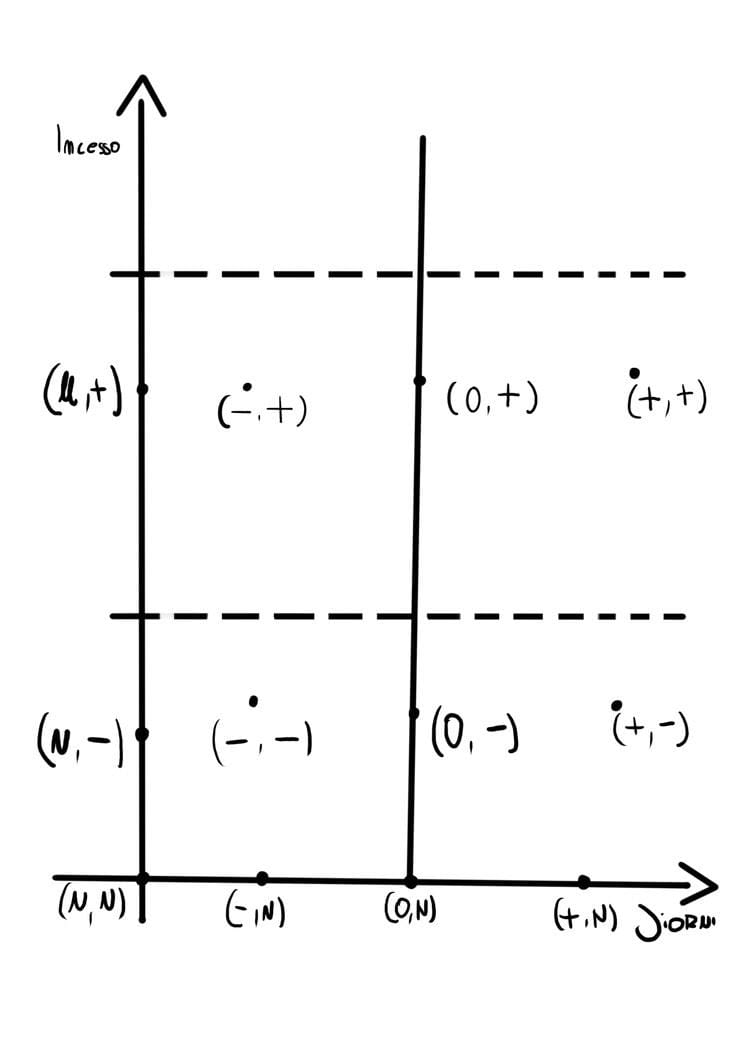
\includegraphics[scale=0.35]{assets/immagini varie/grafico media.jpeg}
    \caption*{\textbf{Figura}: Prodotto cartesiano CE}\label{fig:CE_graph}
\end{figure}

\vspace{0.2cm}
\begin{lstlisting}[language = Java , frame = trBL , firstnumber = last , escapeinside={(*@}{@*)} , commentstyle=\color{brown}]
public class mediaTest {
/*
   CLASSI DI EQUIVALENZA:

      INCASSO: {NULL, NEGATIVO, POSITIVO}
      GIORNI: {NULL, NEGATIVO, ZERO, POSITIVO}

 --------------------------------------------------------------------------------

   STRATEGIE DI TESTING UTILIZZATE:
      BlackBox e WhiteBox secondo il criterio SECT

     ==== BLACKBOX ====

 ------------------------------------------------------------------------------ */

    StatisticsActivityMock mock;

    @Before
    public void setUp(){
        mock = new StatisticsActivityMock();
    }

    @Test
    public void testMedia(){
        float result = mock.media(17, 50f);
        assertEquals(2.94f, result, 0.001f);
    }
    @Test
    public void testGiornoNegativoIncassoPositivo(){
        assertThrows(IllegalArgumentException.class,
                () -> mock.media(-3, 50.06f)
        );
    }
    @Test
    public void testGiornoPositivoIncassoNegativo(){
        assertThrows(IllegalArgumentException.class,
                () -> mock.media(3, -50.06f)
        );
    }
    @Test
    public void testGiornoEIncassoNegativi(){
        assertThrows(IllegalArgumentException.class,
                () -> mock.media(-3, -50.06f)
        );
    }

    @Test
    public void testGiornoZero(){
        assertAll(
                () ->  assertThrows(ArithmeticException.class,
                        () -> mock.media(0, 50.06f)
                ),
                () ->  assertThrows(ArithmeticException.class,
                        () -> mock.media(0, -50.06f)
                )
        );
    }
\end{lstlisting}
\vspace{0.2cm}

\begin{lstlisting}[language = Java , frame = trBL , firstnumber = last , escapeinside={(*@}{@*)} , commentstyle=\color{brown}]
/*     ==== WHITEKBOX ====

------------------------------------------------------------------------------ */

    @Test
    public void testGiornoNull(){
        Integer giorno = null;
        assertAll(
                () ->   assertThrows(NullPointerException.class,
                        () -> mock.media(giorno, 0.30f)
                ),
                () ->   assertThrows(NullPointerException.class,
                        () -> mock.media(giorno, -0.30f)
                )
        );
    }
    @Test
    public void testIncassoNull(){
        Float incasso = null;
        assertAll(
                () ->   assertThrows(NullPointerException.class,
                        () -> mock.media(0, incasso)
                ),
                () ->   assertThrows(NullPointerException.class,
                        () -> mock.media(3, incasso)
                ),
                () ->   assertThrows(NullPointerException.class,
                        () -> mock.media(-3, incasso)
                )
        );
    }

    @Test
    public void testCampiNull(){
        Integer giorno = null;
        Float incasso = null;
        assertThrows(NullPointerException.class,
                () -> mock.media(giorno, incasso)
        );
    }


}

\end{lstlisting}


